\chapter{Revision Control}

\includegraphics[scale=0.20]{images/owl-50267_1920.jpg}

\justify{}
Using a revision control\index{revision control} methodology allows us to organize and store project artifacts. Multiple users or
teams can collaborate on a single code base. Websites, like \href{https://github.com}{github.com} for example, are foundational to our workflow. They are a key piece of 
our software delivery pipeline since they allow us to declare a single source of truth for the code that makes up our project.

\justify{}
In addition to giving us a way to back up and store our work, essentially for free, revision control facilitates a greater degree
of collaboration. There are other similar, (mostly) free services we can choose from, for example Bit Bucket and Git
Lab. For the purposes of this book we will focus GitHub\index{GitHub}, since it is the most common and well known.

\section{The Relationship Between Git and GitHub}

\justify{}
Git is the tool that allows for revision control of your work. GitHub is a repository for storing that work, creating teams to work on projects, tracking issues, defining release packages,
and more. Simply put, \href{github.com}{github.com} is a website that gives you a place to store the work you are using git to manage. 

\subsection{Enable Two-Factor Authentication}

\justify{}
One of the very first things you should do (after creating an account,
that is) is to configure two-factor authentication (2FA)\index{2FA} for your GitHub account.

\justify{}
Next let's take a look at two of the key methods of interacting with projects and other people on github.com.

\subsection{Forking and Cloning Repositories}

\justify{}
When someone else has a project on github.com that you would like to make changes to,
you can make a ``fork'' of that project. Forking\index{forking} a repository means you
are making a copy of that repository to your personal account on the GitHub web site.

\justify{}
Creating a ``clone''\index{cloning a repo} of your fork to your local machine is done so that
you can make changes without altering the original project before testing and review of the changes takes place.

\justify{}
Adding a ``remote'' is a git convention to easily push changes from your clone back to
the original source repository.

\begin{figure}[!htb]

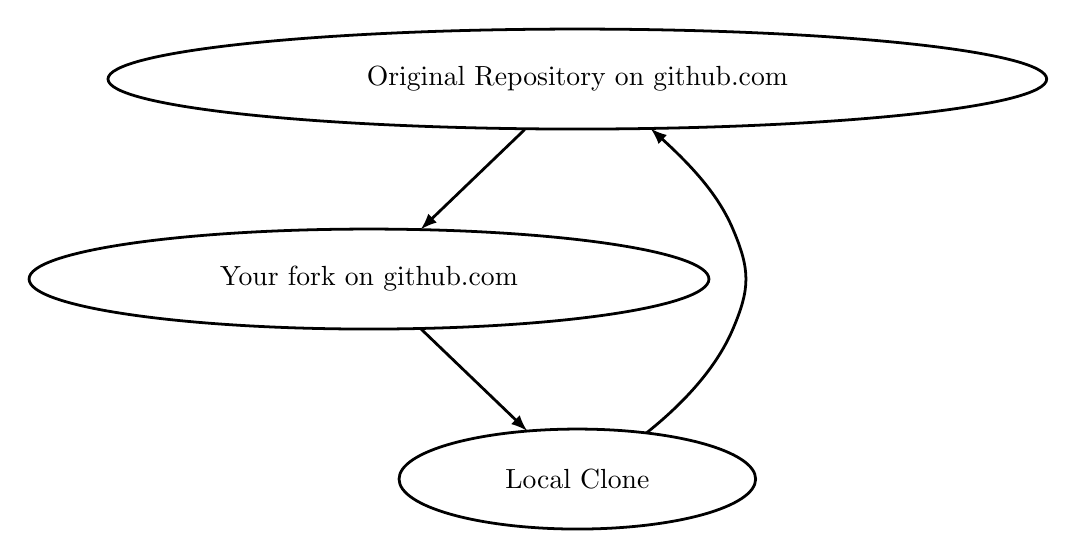
\begin{tikzpicture}[>=latex,line join=bevel,]
  \pgfsetlinewidth{1bp}
%%
\pgfsetcolor{black}
  % Edge: orig -> fork
  \draw [->] (178.26bp,143.83bp) .. controls (169.13bp,135.07bp) and (158.04bp,124.42bp)  .. (140.85bp,107.91bp);
  % Edge: fork -> clone
  \draw [->] (140.73bp,72.202bp) .. controls (150.06bp,63.242bp) and (161.52bp,52.241bp)  .. (179.12bp,35.345bp);
  % Edge: clone -> orig
  \draw [->] (222.15bp,34.664bp) .. controls (233.94bp,44.073bp) and (246.8bp,56.959bp)  .. (253.19bp,72.0bp) .. controls (259.45bp,86.726bp) and (259.45bp,93.274bp)  .. (253.19bp,108.0bp) .. controls (248.45bp,119.15bp) and (240.16bp,129.12bp)  .. (223.62bp,144.15bp);
  % Node: orig
\begin{scope}
  \definecolor{strokecol}{rgb}{0.0,0.0,0.0};
  \pgfsetstrokecolor{strokecol}
  \draw (197.19bp,162.0bp) ellipse (168.97bp and 18.0bp);
  \draw (197.19bp,162.0bp) node {Original Repository on github.com};
\end{scope}
  % Node: fork
\begin{scope}
  \definecolor{strokecol}{rgb}{0.0,0.0,0.0};
  \pgfsetstrokecolor{strokecol}
  \draw (122.19bp,90.0bp) ellipse (122.38bp and 18.0bp);
  \draw (122.19bp,90.0bp) node {Your fork on github.com};
\end{scope}
  % Node: clone
\begin{scope}
  \definecolor{strokecol}{rgb}{0.0,0.0,0.0};
  \pgfsetstrokecolor{strokecol}
  \draw (197.19bp,18.0bp) ellipse (64.19bp and 18.0bp);
  \draw (197.19bp,18.0bp) node {Local Clone};
\end{scope}
%
\end{tikzpicture}


\caption{Forking and cloning.}
\label{forkandclone}
\end{figure}

\justify{}
This can be a tricky pattern to master, but it is fundamental if you
want to join the ranks of Open Source contributors and developers that
enjoy the full power of Git and GitHub.

\paragraph{Steps:}

\begin{itemize}
      \item
            From the original project page on github.com, click the ``fork'' button.
            \begin{itemize}
                  \item
                        This creates a copy of the original repository on your personal
                        GitHub page.
            \end{itemize}
      \item
            Now from your page, make a clone of that fork from github.com to your
            machine.
      \item
            This will allow you to add, update and test code and documentation without altering the original project.
      \item
            On your local machine, create a ``remote'' connection back to the
            original repo.
\end{itemize}

To create a ``remote'' called upstream from your clone to the original
repo, use this example command:

\begin{mybox}{\thetcbcounter: Create Upstream Remote}
git remote add upstream git@github.com:hotpeppersec/devsecops.git
\end{mybox}
\justify{}
After completing these steps you can easily submit pull requests (PRs)
back to the original project.

\hypertarget{keeping-a-clone-in-sync}{%
      \subsection{Keeping a Clone in Sync}\label{keeping-a-clone-in-sync}}

\justify{}
The process of performing a pull request (PR) and merging changes is
covered fairly extensively on the Web. Let's take a quick look at how to
keep your local clone of a repository, as well as your clone on
github.com, up to date.

\hypertarget{steps-1}{%
      \paragraph{Steps}\label{steps-1}}

\justify{}
These are the steps to take once your pull request is merged to the main
branch in the main project repository. From the command line on the
machine where your clone resides:

\begin{itemize}
      \item
            git checkout master
      \item
            git fetch upstream
      \item
            git rebase upstream/master
      \item
            git push origin master
\end{itemize}
\subsection{Creating Repositories}
\justify{}
If you are starting out on a new project, simply creating a repo is
probably enough. Often I will start a repository on my personal account
while I use the steps in this book to get the project off the ground.
Later I will move the repository into an organization where the
responsibility for ownership and administration can be shared with other
folks.

\justify{}
While the repository is owned by me, I use a much simpler process for
managing my code check-ins.

\hypertarget{steps-2}{%
      \paragraph{Steps}\label{steps-2}}

\begin{itemize}
      \item
            Create the repository on github.com from my personal account.
      \item
            Make a clone of that new repository from github.com to my local host.
      \item
            Do my pull requests and merges as desired.
      \item
            Do a git pull to my master branch to keep my local clone up to date.
\end{itemize}
\subsection{Example Repository}
\justify{}
A GitHub Template Repository is available should you decide to follow
along with the code examples in this book. The next sets of steps are
predicated on having Docker installed and running as described in the
previous chapter.

\paragraph{Template Steps}
\begin{itemize}
      \item
            Navigate to ``https://github.com/hotpeppersec/rapid\_secdev\_framework''
      \item
            Click the green button ``Use this template''
      \item
            Select a repository name, like ``devsecops'' for
            example.
      \item
            Now click ``Create repository from template''
\end{itemize}

\justify{}
Now you have a repository in your GitHub account that you can use for
testing and completing lab examples detailed in this book. For our first
exercise, let's try to make a clone of the repository we generated from
template.


\paragraph{Cloning Steps}

\begin{itemize}
      \item
            Navigate to the main page for our new repository on github.com.
      \item
            \begin{description}
                  \item[Clone the repository to your local host by clicking on the green
                        ``Clone or download'' button.]
                        \begin{itemize}

                              \item
                                    Be sure to clone with ``SSH'' and not ``HTTPS''.
                        \end{itemize}
            \end{description}
      \item
            Change to the clone directory with the ``cd'' command.
\end{itemize}

\justify{}
From the devsecops directory, execute the command
``make docker'' to get to a command prompt within the container.
\justify{}
Consider the following example. Notice that the command prompt changes
to indicate that you have a BASH shell in the running container.

\begin{mybox}{\thetcbcounter: Output from make docker command}
  \lstinputlisting{code/github/make-docker-output.txt}
\end{mybox}

\subsection{CODEOWNERS}

\justify{}
Creating a CODEOWNERS\index{CODEOWNERS} file
is a good way to automatically tag folks in PRs to make them aware of
changes to certain files or folders in your projects.

\justify{}
In it's most basic form, the CODEOWNERS file in the .github directory
simply lists the file(s) and the owner(s) on a line together.

\justify{}
Consider this example where we add the @hotpeppersec to the CODEOWNERS
file.

\begin{mybox}{\thetcbcounter: Adding a user to CODEOWNERS file}
      \lstinputlisting{code/github/create-codeowners.txt}
\end{mybox}
\justify{}
In this example, the @githubusername user will be tagged as a reviewer
in all pull requests.

\subsection{The .gitignore file}
\justify{}
Use this file\index{.gitignore} to designate items that should be excluded from revision
control. This is useful for helping keep credentials and other secrets
out of the GitHub repository.

\justify{}
Consider the following example .gitignore file. This will prevent you
from checking in the .DS-Store that Macintosh creates in many folders.

\begin{mybox}{\thetcbcounter: Example .gitignore file}
      \lstinputlisting{code/github/create-gitignore.txt}
\end{mybox}

\subsection{Working with Branches}
\justify{}
Naming your branches something useful is helpful (self documenting). Let's look at how
to create a branch.

\hypertarget{steps-3}{%
      \paragraph{Steps}\label{steps-3}}

\subsection{Pull Requests}
\justify{}
When you make changes on a local branch, say on your personal laptop,
you will eventually want those changes to flow back into the main
project. Opening a pull request\index{Pull Request} is a means of letting other
people know you've got a set of changes ready for review and potential changes.

\justify{}
Keeping pull requests smaller and more frequent makes it easier for your
peers to review your changes. It also means you will be less likely to lose work.
\justify{}
Let's use our changes to the CODEOWNERS file to try making a change in
our clone of the repository in GitHub, then pushing that change up to
the repository.

\hypertarget{steps-4}{%
      \paragraph{Steps}\label{steps-4}}

\begin{itemize}
      \item
            Create a new branch, for example git checkout -b newbranch
      \item
            Create the .github directory if it does not exist, then the CODEOWNERS
            file in that directory.
      \item
            Use git to add the file to the commit: git add CODEOWNERS
      \item
            Commit the file with git, git commit -S -m `add CODEOWNERS file'
      \item
            Push this commit to github.com, git push origin newbranch
      \item
            Use the github.com website to open and merge the pull request.
\end{itemize}
\subsection{Repository Settings}
\justify{}
When setting up a new repository in my GitHub account, I always click
the Settings tab (with the little gear icon) and then choose the
``Branches'' section. The Default branch gets set to ``main''. Clicking
the ``Add Rule'' button, entering ``main'' for the ``Branch name pattern'',
and then the green ``Create'' button sets up master as a protected branch.
Consider the following example {myFig2}.
\begin{figure}
      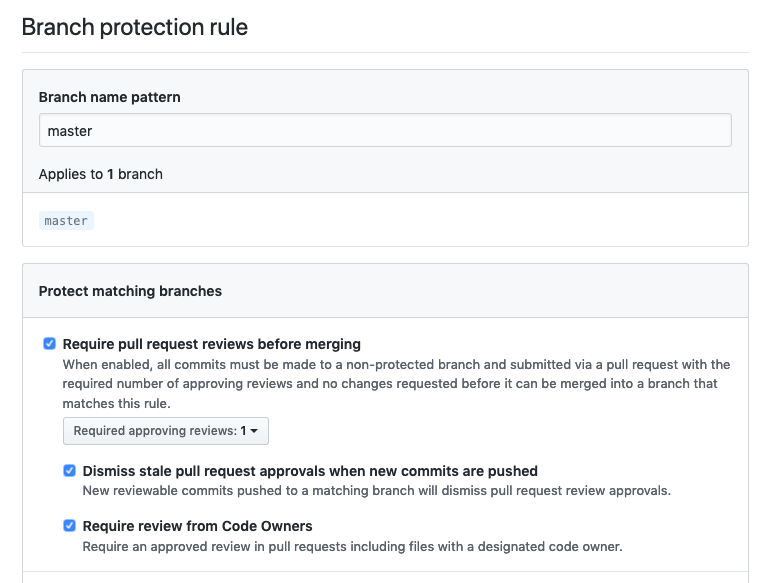
\includegraphics[scale=0.50]{images/github-branch-protection.png}
      \caption{Setting up branch protection.}
      \label{branchprotect}
\end{figure}

\justify{}
After we start to work with CI/CD tools (status checks, like GitHub
Actions for example) new choices ({myFig3}) become available in this
part of your repository for managing those checks.

\begin{figure}
      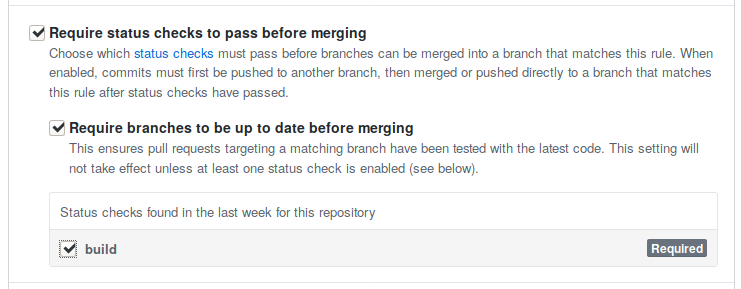
\includegraphics[scale=0.53]{images/guthub-status-check.png}
      \caption{Requiring status checks.}
      \label{statuscheck}
\end{figure}

\subsection{Automated Repository Scanning}
\justify{}
There are many GitHub plugins that are free for
single-user/non-commercial scenarios. a cursory search of the web of the
GitHub Marketplace will turn up many of these. Let's leave some of the
tedious work to the bots, allowing us to focus on our DevSecOps journey to the cloud!

\subsubsection{Renovate}
\justify{}
WhiteSource Renovate is what's known as a dependency scanner. It is free
for single user to add from the GitHub Marketplace. It can tell you when you are using
a version of a module or image that
is out of date. For example, if you have a Dockerfile that specifies
Python 3.8.1, Renovate will open a pull request on your repository to
update the version string in that Dockerfile to the most current version
available. You can also grant Renovate the permissions required to
simply merge the change with no human interaction. Renovate supports
JavaScript, Java, Ruby, PHP, Python, Go, Cargo, Elixir, Docker, and
more.

\justify{}
Once you've signed up and specified which repositories you want Renovate
to monitor, it opens a pull request to install a simple default
configuration file called renovate.json. Merge this initial pull request
and you're up and running!

\subsubsection{LGTM}
\justify{}
Semmle is a company that runs a code scanning service we can use to keep
an eye on our repositories for issues with syntax and dependencies. It
is tightly coupled with github.com and can be configured from lgtm.com
after logging in with your GitHub credentials.
\justify{}
As a fun aside, LGTM stands for ``looks good to me'', something developers
will add as review comments when their pull request is simple or matches
obvious expectations.
\clearpage
\section{Directory Structure}
\justify{}
Relevant files and folders mentioned in this chapter are organized as
seen below.

\begin{figure}[!htb]
      \centering
      
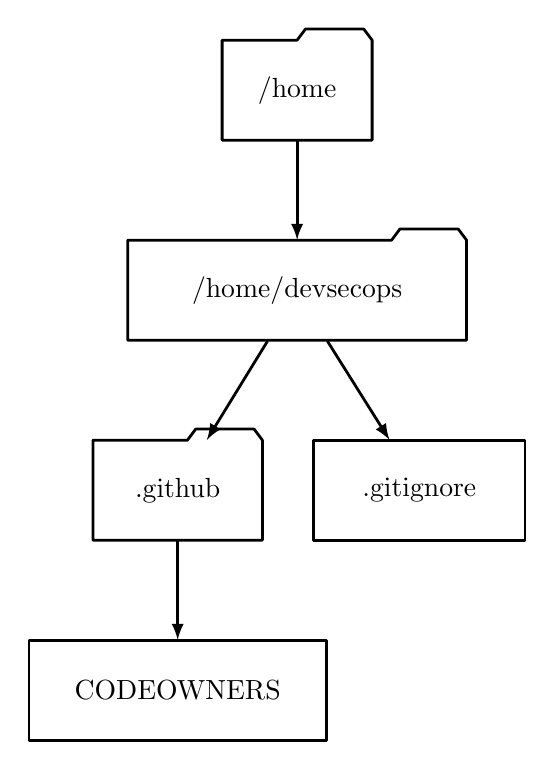
\begin{tikzpicture}[>=latex,line join=bevel,]
  \pgfsetlinewidth{1bp}
%%
\pgfsetcolor{black}
  % Edge: home -> devsecops
  \draw [->] (96.5bp,215.7bp) .. controls (96.5bp,207.98bp) and (96.5bp,198.71bp)  .. (96.5bp,180.1bp);
  % Edge: devsecops -> github
  \draw [->] (85.871bp,143.7bp) .. controls (80.872bp,135.56bp) and (74.809bp,125.69bp)  .. (64.007bp,108.1bp);
  % Edge: devsecops -> gitignore
  \draw [->] (107.38bp,143.7bp) .. controls (112.49bp,135.56bp) and (118.7bp,125.69bp)  .. (129.75bp,108.1bp);
  % Edge: github -> codeowners
  \draw [->] (53.5bp,71.697bp) .. controls (53.5bp,63.983bp) and (53.5bp,54.712bp)  .. (53.5bp,36.104bp);
  % Node: home
\begin{scope}
  \definecolor{strokecol}{rgb}{0.0,0.0,0.0};
  \pgfsetstrokecolor{strokecol}
  \draw (123.5bp,252.0bp) -- (120.5bp,256.0bp) -- (99.5bp,256.0bp) -- (96.5bp,252.0bp) -- (69.5bp,252.0bp) -- (69.5bp,216.0bp) -- (123.5bp,216.0bp) -- cycle;
  \draw (96.5bp,234.0bp) node {/home};
\end{scope}
  % Node: devsecops
\begin{scope}
  \definecolor{strokecol}{rgb}{0.0,0.0,0.0};
  \pgfsetstrokecolor{strokecol}
  \draw (157.5bp,180.0bp) -- (154.5bp,184.0bp) -- (133.5bp,184.0bp) -- (130.5bp,180.0bp) -- (35.5bp,180.0bp) -- (35.5bp,144.0bp) -- (157.5bp,144.0bp) -- cycle;
  \draw (96.5bp,162.0bp) node {/home/devsecops};
\end{scope}
  % Node: github
\begin{scope}
  \definecolor{strokecol}{rgb}{0.0,0.0,0.0};
  \pgfsetstrokecolor{strokecol}
  \draw (84.0bp,108.0bp) -- (81.0bp,112.0bp) -- (60.0bp,112.0bp) -- (57.0bp,108.0bp) -- (23.0bp,108.0bp) -- (23.0bp,72.0bp) -- (84.0bp,72.0bp) -- cycle;
  \draw (53.5bp,90.0bp) node {.github};
\end{scope}
  % Node: gitignore
\begin{scope}
  \definecolor{strokecol}{rgb}{0.0,0.0,0.0};
  \pgfsetstrokecolor{strokecol}
  \draw (178.5bp,108.0bp) -- (102.5bp,108.0bp) -- (102.5bp,72.0bp) -- (178.5bp,72.0bp) -- cycle;
  \draw (140.5bp,90.0bp) node {.gitignore};
\end{scope}
  % Node: codeowners
\begin{scope}
  \definecolor{strokecol}{rgb}{0.0,0.0,0.0};
  \pgfsetstrokecolor{strokecol}
  \draw (107.0bp,36.0bp) -- (0.0bp,36.0bp) -- (0.0bp,0.0bp) -- (107.0bp,0.0bp) -- cycle;
  \draw (53.5bp,18.0bp) node {CODEOWNERS};
\end{scope}
%
\end{tikzpicture}


      \caption{GitHub related files.}
      \label{githubfiles}
\end{figure}
